\documentclass[aps,prb,onecolumn,nofootinbib,superscriptaddress]{revtex4-2}
\usepackage{amsmath,amssymb,amsthm,mathtools,bm}
\usepackage{booktabs}
\usepackage[colorlinks=true,linkcolor=blue,citecolor=blue,urlcolor=blue]{hyperref}
\usepackage{microtype}
\usepackage{graphicx}

\newtheorem{proposition}{Proposition}
\newtheorem{definition}{Definition}
\newcommand{\Gr}{\operatorname{Gr}}
\newcommand{\Span}{\operatorname{span}}
\newcommand{\tr}{\operatorname{tr}}
\newcommand{\cH}{\mathcal H}
\newcommand{\cF}{\mathcal F}
\newcommand{\cE}{\mathcal E}
\newcommand{\cM}{\mathfrak M}

\begin{document}
\title{Constraint-flag breakdown for finite-support optimal-Wannier resets:\\a preregistered CPU pilot}
\author{A. Bhuiyan}
\affiliation{Department of Physics}
\date{August 17, 2026}

\begin{abstract}
We formulate a finite-size diagnostic for the obstruction encountered when an adaptive
Gaussian circuit attempts to impose a redundant word of compactly truncated
optimal-Wannier (OW) occupation constraints.  Filled and empty reset modes generate two
increasing subspace flags and hence a decreasing filtration of compatible half-filled
Grassmannians.  Exact failure is detected by a rank bound or a nonzero principal angle
overlap; approximate failure is quantified by a Ky Fan minimum-frustration functional.
We sharply separate this static completion problem from a cumulative tangent-kernel flag
and from the dynamical loss of a reset constraint upon its next visit.  A preregistered
$16\times20$ CPU pilot compares a support-terminated domain-wall slab to a periodic
uniform control under random and raster schedules.  The construction evades no known
no-go theorem: finite support removes the exponentially localized common dark state
required for exact pure Chern preparation, while the conditional trajectory ensemble
and unconditional mixed state are logically distinct objects.
\end{abstract}

\maketitle
\setcounter{tocdepth}{2}
\tableofcontents

\section{Premise and relation to the dissipative no-go theorem}

An exactly flat Chern band admits exponentially localized OW modes but no translation-
covariant compactly supported orthonormal Wannier basis.  Goldstein's dissipative no-go
theorem makes the corresponding preparation tension operational: a finite-range,
number-conserving quadratic Lindbladian cannot simultaneously have a unique pure Chern
steady state and a size-independent dissipative gap under its stated regularity
assumptions~\cite{Goldstein2019}.  Our circuit uses finite $n_{\rm shell}$ truncations of
otherwise exponential OW tails.  Those compact controller modes need not share any
exact half-filled Gaussian dark state.  Perfect correction resets the mode selected at
the current letter; it does not make all earlier nonorthogonal occupation constraints
simultaneous constants of motion.

There is therefore no evasion of the obstruction.  At finite support, one relinquishes
the common exact pure Chern fixed point.  Along a conditioned trajectory the state
remains Gaussian and pure after the measurement/reset record is specified, whereas the
unconditional state is a record average and is generally mixed.  In a hard-wall slab,
the slowest restoration scale may also close with system size.  The present experiment
asks where this incompatibility first becomes visible and whether its excess is
localized at the support-termination boundary.  It does \emph{not} use overlap winding
as the compact mode's Chern number.

\section{Filled/empty flags and compatible completions}

Let $\cH\simeq\mathbb C^D$ be the active one-body space and let a circuit word be
$(w_j,s_j)_{j=1}^M$, where $\lVert w_j\rVert=1$ and $s_j\in\{0,1\}$ is the target
occupation.  Define the increasing flags
\begin{equation}
 \cF_m=\Span\{w_j:s_j=1,\ j\le m\},\qquad
 \cE_m=\Span\{w_j:s_j=0,\ j\le m\}.
\end{equation}
A pure number-conserving Gaussian state with $N$ particles is an occupied plane
$U\in\Gr(N,D)$, or equivalently a rank-$N$ orthogonal projector $P_U$.  Its compatible
set after the first $m$ letters is
\begin{equation}
 \cM_m=\{U\in\Gr(N,D):\cF_m\subseteq U\subseteq\cE_m^\perp\}.
\end{equation}
Thus $\cM_{m+1}\subseteq\cM_m$: the word generates a decreasing Grassmannian
filtration even though $\cF_m$ and $\cE_m$ increase.

\begin{proposition}[Exact completion]
The prefix admits a rank-$N$ completion if and only if
\begin{equation}
 \cF_m\perp\cE_m,
 \qquad \dim\cF_m\le N\le D-\dim\cE_m.
 \label{eq:completion}
\end{equation}
\end{proposition}
\begin{proof}
Necessity follows because $\cF_m\subset U$ and $\cE_m\subset U^\perp$.  Conversely,
orthogonality gives $\cF_m\subset\cE_m^\perp$.  The rank bounds ensure that one may
choose an $(N-\dim\cF_m)$-plane in
$\cE_m^\perp\ominus\cF_m$ and append it to $\cF_m$.
\end{proof}
The exact breakdown letter is
\begin{equation}
 m_\star=\min\{m:\cM_m=\varnothing\}.
\end{equation}
With orthonormal span matrices $Q_{F,m}$ and $Q_{E,m}$, nonorthogonality is diagnosed by
$\sigma_{\max}(Q_{F,m}^\dagger Q_{E,m})>0$.  We also record the total principal-angle
overlap
\begin{equation}
 \Phi_m=\lVert Q_{F,m}^\dagger Q_{E,m}\rVert_F^2=\sum_a\cos^2\theta_a.
\end{equation}

\section{Minimum frustration and marginal cost}

Exact feasibility is numerically brittle and deliberately binary.  For normalized
constraints and nonnegative weights $\gamma_j$, define
\begin{equation}
 F_m(P)=\sum_{j\le m}\gamma_j\big[s_j(1-\langle w_j,Pw_j\rangle)
 +(1-s_j)\langle w_j,Pw_j\rangle\big],\qquad P^2=P=P^\dagger,
\quad\tr P=N.
\end{equation}
Writing
$A_m=\sum_{j\le m}\gamma_j(1-2s_j)|w_j\rangle\langle w_j|$, the Ky Fan principle gives
\begin{equation}
 F_\star(m)=\sum_{j\le m}\gamma_js_j+\sum_{a=1}^{N}\lambda_a^\uparrow(A_m),
 \qquad \Delta_m=F_\star(m)-F_\star(m-1)\ge0.
 \label{eq:kyfan}
\end{equation}
The implementation updates numerical span bases and rank conditions at every letter.
It evaluates principal spectra and Eq.~\eqref{eq:kyfan} at preregistered block, shell,
column, and random-word decile checkpoints; at each such $m$, $F_\star(m-1)$ is also
evaluated so the reported $\Delta_m$ is the literal one-letter marginal.

\section{Three objects that must not be conflated}

The \emph{static constraint flag} above asks for a simultaneous Gaussian completion of
a finite word.  A distinct \emph{cumulative tangent-kernel flag} is formed from kernels
of linearized measurement/reset maps acting on covariance perturbations.  Its rank loss
measures erased tangent directions and can be studied later, but is not inferred here.
Finally, \emph{dynamical reset retention} is a revisit statistic.  Immediately before
the next imposition of letter $j$ in cycle $t$, let
\begin{equation}
 \epsilon_{j,t}=1-p_{\rm target}(j,t).
\end{equation}
The observed wrong outcome $X_{j,t}\in\{0,1\}$ obeys
$\mathbb E[X_{j,t}\mid\mathcal F_{t^-}]=\epsilon_{j,t}$.  Therefore
$1-\epsilon$ is retention, and $\langle X\rangle=\langle\epsilon\rangle$ is a mandatory
calibration check rather than an additional physical hypothesis.  Static
incompatibility does not by itself imply persistent stationary activity.

\section{Preregistered CPU protocol}

The production pilot uses $N_x\times N_y=16\times20$, $n_{\rm shell}=1$, perfect
correction, and the maximally mixed initial covariance.  The hard support-terminated
wall has active centers $x=3,\ldots,13$; the static uniform comparison uses the same
centers but retains the full periodic one-body basis.  Static $n_{\rm shell}=2$ and
untruncated frames are convergence controls.  We order constraints from interior shells
to the walls, in raster-$y$ order, and by each saved first-cycle random word.

Dynamics compare the wall and uniform geometries under random and raster-$y$ schedules.
Ten root seed IDs are reused across configurations and are called \emph{matched-seed}
IDs, not identical records, because active words differ.  Each trajectory has 80 cycles;
cycles 1--40 are burn-in.  The statistical unit is the trajectory, never the individual
site/channel revisit.  We report paired matched-seed and unpaired trajectory-bootstrap
intervals, left/right wall regions, the interior, channel and position in the word, and
uniform pseudo-interfaces at $x=3,13$.

\section{Promotion rule and limitations}

GPU/Colab work is recommended only if all of the following hold: (i) a reproducible
static marginal-frustration excess begins when boundary shells enter; (ii) it is present
at both walls and above the uniform finite-shell background; (iii) post-burn-in revisit
loss is greater at both wall interfaces than in the wall interior for both schedules;
(iv) uniform pseudo-interfaces have no comparable peak; and (v) signs survive both
matched-seed and unpaired trajectory bootstrap analyses.  Otherwise the pilot is
reported as null or schedule-dependent and no GPU campaign is started.

A flag defect is not by itself proof of topology, chirality, a compact-mode Chern
number, or stationary activity.  Finite size, the chosen OW gauge, support termination,
and schedule all remain possible sources of structure.  The experiment resolves a
specific compatibility mechanism, not an invariant classification.

\section{Generated pilot result}

\providecommand{\PilotStatus}{completed}
\providecommand{\PilotVerdict}{\texttt{NULL\_OR\_SCHEDULE\_DEPENDENT\_NO\_GPU}}
\providecommand{\PilotParameters}{$16\times 20$, 10 matched seed IDs, 80 cycles, burn-in 40}
\begin{table}[ht]
\centering
\caption{Post-burn-in wall interface-minus-interior revisit loss. Confidence intervals resample trajectories.}
\begin{tabular}{lcc}\toprule
schedule & estimate & 95\% CI \\\midrule
random & 0.04481 & [0.04441,0.04524] \\
raster\_y & 0.0429 & [0.04239,0.04336] \\
\bottomrule\end{tabular}
\end{table}
\begin{figure}[ht]\centering
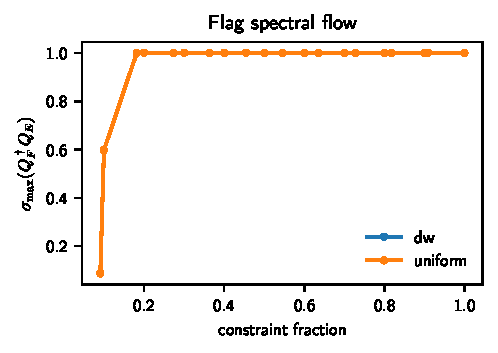
\includegraphics[width=0.72\linewidth]{generated/flag_spectral_flow.pdf}
\caption{Static filled/empty flag spectral flow. This overlap diagnostic is not a Chern-number estimator.}
\end{figure}
\begin{figure}[ht]\centering
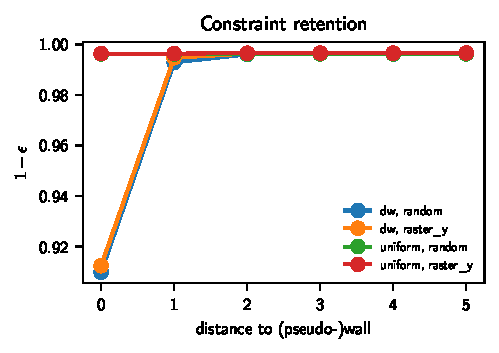
\includegraphics[width=0.72\linewidth]{generated/retention_profiles.pdf}
\caption{Post-burn-in reset-retention profiles. Static incompatibility and stationary activity are tested separately.}
\end{figure}


Status: \PilotStatus.  Parameters: \PilotParameters.  Gate verdict: \PilotVerdict.

\begin{thebibliography}{9}
\bibitem{Goldstein2019}
G.~Goldstein, ``Dissipation-induced topological insulators: A no-go theorem and a
recipe,'' SciPost Phys. \textbf{7}, 067 (2019).
\end{thebibliography}

\end{document}
